% jan 15 10 jh: have check edall seisan.def against libsei,please add definitiopns, change all lower case to upper case
% may 2 2012 jh: add comment about multiple users


%\chapter{INSTALLATION}
\chapter{Installation}
\label{chap:installation}

SEISAN has been tested and compiled for Windows 2000/XP, 
Solaris, Redhat Linux and MacOSX.

\textbf{Upgrade from version 7.0 or higher}

Before you start, take a backup copy of your DAT directory. Note that 
when you upgrade, many parameter files will be overwritten so make 
sure old parameter files are copied before putting in a new version 
of SEISAN. The most important are in DAT: 
\texttt{STATION0.HYP, SEISAN.DEF, MULPLT.DEF}. 
Also the Unix setup file 
%\textcolor{red}{lo-change: 
SEISAN.csh and SEISAN.bash is overwritten. 
You may also want 
to keep copies of PRO, LIB and INC to keep a copy of the old source 
code, especially if you have done any modifications to the code. 
You can keep almost all of your parameter files, only \texttt{SEISAN.DEF} 
has been changed. Check this file and change to your system. Some individual program parameter files like for SPEC have changed. 

\textbf{How to get SEISAN}

SEISAN can be copied from \texttt{ftp.geo.uib.no} (\texttt{129.177.55.4}), 
login is ftp and password is your email address or from 
%\url{http://www.geo.uib.no/seismo/software/seisan.html} (or 
\url{https://www.uib.no/rg/geodyn/artikler/2010/02/software}
%\texttt{129.177.55.5} instead of \newline
%\texttt{www.geo.uib.no}). 
On the 
AFTP server go to \texttt{/pub/seismo/SOFTWARE/SEISAN}. Use binary 
mode for the compressed files (tar and zip). Before copying, check 
the readme file for latest updates, changes and current content of 
the directory. The directory will at least contain the following files: 

\begin{tabular}{|lp{10cm}|}
\hline
\texttt{seisan\_X.Y\_.unix.tar.gz} & a compressed tar file, whole 
distribution with executables and test data, X.Y 
stands for the latest distribution number and Unix for the respective Unix 
system (solaris or linux). \\
\texttt{seisan.\_X.Y.exe}  & Windows distribution an install file \\
\texttt{seisan\_X.Y.pdf}  & The SEISAN manual, Adobe PDF \\
\texttt{seitrain\_X\_Y.pdf} & SEISAN training course \\
\texttt{testdata\_X.Y.tar.gz} & SEISAN data for the training course\\
\hline
\end{tabular}
\newline

Alternatively SEISAN might be obtained on a CD with the same content as 
above (write to \newline
\texttt{jens@geo.uib.no}). 

Section \ref{sect:compiling} gives additional information about modifications and recompilation. 

\section{Unix (SOLARIS and Linux)} 
\label{sect:instal-unix}

\textbf{Solaris:} The SEISAN programs have been compiled on Solaris 7 using Sun Workshop 5, which means you have to recompile if you use an earlier version of the operating system or compiler. If you can recompile on Solaris, please do so! The programs on Solaris are compiled dynamically, which means not all system and compiler libraries are included in the executables. If you are running Solaris, the system libraries are normally installed, but the Sun system compilers might not be installed. If the compilers are not installed, you have the following options: (1) you install the Sun workshop compilers, license is not needed, since only the libraries are required; (2) you install the required libraries, which are part of the Solaris SEISAN distribution (instructions below).  

\textbf{Linux:} The programs have been compiled under Redhat Linux7.2 
using the GNU compilers gcc and g77. It is recommended to recompile 
the programs, since otherwise the programs might not run on your 
Linux distribution. In the Redhat distribution of Linux the Fortran 
compiler is not part of the standard distribution, it has to be 
installed (see your Linux manual for instructions). 
THE USER ACCOUNT MUST BE SET UP TO USE csh, tcsh (use SEISAN.csh) or bash (use SEISAN.bash),
in order for the SEISAN scripts to work. 
Note that in the following SEISAN.csh stands for both SEISAN.csh and SEISAN.bash.
Otherwise the scripts need to be adopted to the shell used.


\textbf{Instructions}

The first step is to install the distribution, the procedure is the same for all Unix platforms. 

1.  Get tar file 

Copy the distribution file for your platform from CD or transfer it 
through FTP or from the web site to the SEISAN top directory, 
this could be a directory \texttt{seismo} under the home directory. 

2.  Decompress 

%\textcolor{red}{lo-change:}
\texttt{gunzip seisan\_\textit{version}\_\textit{system}.tar.gz}

There should now be the uncompressed file in your directory (without \texttt{.gz}). 

3. Install SEISAN 

\texttt{tar xvf seisan.tar}

Check that the SEISAN directories have been created. 

If SEISAN has been installed without executable files, they can all be generated with the command `make all' from the PRO directory. On Sun this requires that the Sun compilers be installed, on Linux/MacOSX it requires the GNU Fortran compilers (g77, only gcc before version 4.0; now gfortran). See also section on compilation (\ref{sect:compiling}). 

Install Workshop libraries 

In the SUP directory of the Solaris distribution the file 
\texttt{sun\_ws\_lib.tar.Z} 
includes the libraries that are needed to run SEISAN on Solaris in 
case the compilers are not installed. The file is a compressed tar file. 
The files can be extracted with \texttt{uncompress sun\_ws\_lib.tar.Z} 
and then \texttt{tar xvf sun\_ws\_lib.tar}. The library files can be 
stored in any directory in the system, but the environmental 
variable \texttt{LD\_LIBRARY\_PATH}
\index{LD\_LIBRARY\_PATH} has to be set accordingly. 
If you are using the C-shell, this can be done by adding to 
the \texttt{.cshrc} file the line 
\texttt{setenv LD\_LIBRARY\_PATH /path/:\$LD\_LIBRARY\_PATH}. 
This would add \texttt{/path/} (which is the path to where the libraries are) 
to \texttt{LD\_LIBRARY\_PATH}, which normally is already defined. 

4. Set system parameters 

If you are doing an update, some of the following settings can be skipped. 

Activate SEISAN:\newline
\textbf{csh/tcsh shell} :\newline
In your .cshrc file, the aliases and paths used by SEISAN are defined 
by adding the line \newline
\texttt{source /home/seismo/COM/SEISAN.csh} \newline
where 
\texttt{../seismo} is the directory below which SEISAN has been installed. 
The \texttt{SEISAN.csh} script file assumes that you are running either csh or 
tcsh as your shell. \newline
\textbf{bash shell} :\newline
%\textcolor{red}{pv-change: 
If you are using the \index{Bash shell} bash shell add this line to your 
\texttt{.bashrc} file :\newline
\texttt{. /home/seismo/COM/SEISAN.bash} \newline
bash might include a 
\texttt{select} program, if that is the case on your pc you also need to add this 
line in your 
\texttt{.bashrc} file :\newline
\texttt{alias select="/home/seismo/PRO/select"} \newline
to use the SEISAN SELECT program.
%}
 \newline
If you are using another shell you need to modify the script 
accordingly or change the shell. It is assumed that 
\index{X Windows}X-windows is installed. 

SEISAN path for programs:\newline
In order for programs and subroutines to know the path to the SEISAN program directory, this must be defined in the file \index{SEISAN.csh}\index{SEISAN.bash}.SEISAN \index{SEISAN\_TOP}in COM. Edit that file and set the \index{Environmental variable}environmental variable SEISAN\_TOP to the name of the \index{Top directory}top directory, meaning the directory structure below and including seismo e.g. /top/users/seismo. This variable is then used to set the path to SEISAN directories. 

Search path for libraries:\newline
To run the NANSEI\index{NANSEI} conversion program under Solaris, the SEISAN LIB directory needs to be included in the environmental variable LD\_LIBRARY\_PATH\index{LD\_LIBRARY\_PATH}. The LIB directory as default is already added to the library search path in the SEISAN.csh file. 

SEISAN path for databases, parameter files etc:\newline
The SEISAN database can be under the same top directory as programs, however it can also be different. This is practical if several users have their own databases, but use the same software. Set environmental variable \index{SEISAN\_TOP}SEISAN\_TOP to top directory e.g. /top/users/seismo. 

%Java settings:\newline
%Aliases are defined to run the Java tools jseisan, seisconf and sformat. The setup in the SEISAN.csh file as default is:\index{Java, start command}\index{jseisan}\index{seisconf}\index{sformat}
%\begin{small}
%\begin{verbatim}
%alias jseisan 'java -DSEISAN\_TOP=\$SEISAN\_TOP -classpath \$SEISAN\_TOP/PRO/jseisan.jar SEISAN'
%alias seisconf 'java -DSEISAN\_TOP=\$SEISAN\_TOP -classpath \$SEISAN\_TOP/PRO/jseisan.jar SEISCONF'
%alias sformat 'java -DSEISAN\_TOP=\$SEISAN\_TOP -classpath \$SEISAN\_TOP/PRO/sformat.jar Sformat'
%\end{verbatim}
%\end{small}
%These settings may have to be changed in case you want to keep the jar files in some other directory. The CLASSPATH (which is used to search for classes) is also modified to include PRO and PRO/jseisan.jar, although this is not needed when using the aliases. 

SEISAN \index{Agency}agency:\newline
In SEISAN.csh also set the environmental variable AGENCY (upper case) to your 3-letter agency code (upper case). This variable is only used by program MACROIN from EEV in connection with entering macroseismic data so for most users ignore this setting. 

SEISAN default database:\newline
To locate the default database directory (here BER) set environmental variable DEF\_BASE in SEISAN.csh. If not set, the name AGA is used. The data bases are found under SEISAN\_TOP. 

SEISAN \index{Editor}editor used in EEV:\newline
The default editor is vi, any other editor can be set with the environmental variable \index{SEISAN\_EDITOR.}SEISAN\_EDITOR. 

SEISAN calibration file directory:\newline
By default, calibration files are in CAL, but they can be in a directory set with variable \index{LOCAL\_CAL}LOCAL\_CAL. The directory name must be complete like /home/users/calibration/ 

SEISARCH\index{SEISARCH}\newline
Gives the architecture, can be either solaris, linux or windows. Used in Makefile when compiling. 

SACAUX\index{SACAUX}\newline
Path to SAC aux directory, required by the SAC routines  for reading and writing, although not really used. 

SACLIB\index{SACLIB}\newline
Specify path and filename to SAC libraries, only needed when you compile programs (Unix) and you have the libraries installed on your system. 

\index{Printer}Printer for Postscript plots:\newline
The \index{Hard copy files}hard copy files from programs are sent to the printer from within the programs using the standard lpr command. In the SEISAN.csh file, define lpr using the standard environmental variable PRINTER. Remember that the printer must accept \index{Postscript}Postscript. PostScript files can also be viewed and printed on most printers outside SEISAN using GhostView, however in that cases files cannot be printed from within a program. 

Scaling for Postscript plots:\newline
By default, plots will be in A4 size. This can be changed by setting 
the environmental variables \newline
SEISAN\_PSSCALE\_X and SEISAN\_PSSCALE\_Y. The default for A4 size 
is 1.0 for both variables. For Letter size the Y-scaling can be set to 0.9. 

Seisan Extension\index{Seisan extension}: \newline
User specific code can be implemented by making use of the environmental 
variable SEISAN\_EXTENSION. The idea is that programs read this variable, 
if set to the user specific string, the user's source code will be 
used instead of the default. An example could be the computation of 
error ellipses. Currently used codes are: BGS. 

4. Testdata The testdata set can be extracted from the file 
\texttt{testdata\_X.Y.tar.Z}. Use programs uncompress and tar to 
extract the data in the SEISAN top directory (keep subdirectory structure). 

\textbf{Dimensions}

Most dimensi\index{Dimension}ons are set in file 
\index{Seidim.inc}\texttt{seidim.inc} in the INC directory. 
In order to change dimensions, first change in the include 
file and then recompile the whole SEISAN distribution. The 
most important dimensions are: \index{Maximum number of traces}

% jh-change: we should consider same dimensions for pc and linux, increase?

\begin{tabular}{|ll|}
\hline
Number of points in one trace & 1 900 000 (1 200 000 on PC) \\
Number of points in memory buffer & 30 000 000 (8 000 000 on PC) \\
Number of lines in NORDIC format file & 4 000 \\
Maximum number of traces in one plot & 1 000 \\
Maximum number of events in one month & 90 000 \\
Maximum number of calibration files & 1 500 \\
%\textcolor{red}{jh-change: 
Maximum number of epicenters in epimap & 90 000 \\
Maximum number of lines in index file made with dirf: & 9 999 \\
\hline
\end{tabular}
\newline

The maximum number of points used by the SEED reading routine 
are set in \texttt{seed\_internal.in.f}. Currently its is set to 1 900 000. 

SEISAN has been tested with much larger dimensions, like 10 000 000 
for number of points in one trace, however large dimensions might 
slow down the speed due to swapping (particularly if memory is not 
large) so a smaller dimension has been chosen. For continuous data, 
SEISAN works with many files so smaller dimensions can be used. For 
the PC version, dimensions may be different from above, check 
\texttt{seidim.inc}. 

\textbf{Note:} In case programs don't work, you might have to recompile, 
see section \ref{sect:compiling}. \newline
%\textcolor{red}{pv-change: 
Some Ubuntu users are missing the 
\texttt{libg2c.so.0} library file, it can be installed with the 
command (you might need to be online):\newline
\texttt{sudo apt-get install gcc} \newline
If this does not work, also try: \newline
\texttt{sudo apt-get install libg2c0}
%}

%\textcolor{red}{pv-change: 
On at \index{64 bit computer} 64 bit computer the IASP files in DAT 
must be regenerated
if you have the files from a 32 bit computer, with the programs \texttt{REMODL} and 
\texttt{SETBRN}
%} 
otherwise \texttt{HYP} will crash.

\textbf{Graphics problem:} \index{Graphics problem on UNIX}
On Solaris, if no colors, make sure color setting is 8 bit. Can be set with 
command m64config -depth 8. See Solaris manual. 

Multiple users on Linux/Unix

If two or more users are working with EEV at the same time with the same user, there is a risk that the S-file names are being mixed up so an event from one year suddenly gets the S-file name from another year. This is caused by both users using the same environmental variable for the S-file (should be changed !). The solution is that each users has his/her own account, which in any case is the most convenient.
index{Problem: S-file changed name}
index{Multiple users on Linux/Unix}
index{Wrong S-file name}
index{S-file changed name}

\section{MacOSX}
\index{MacOSX}

%\textcolor{red}{lo-change: }
The MacOSX version does not come pre-compiled, and will have to be compiled by the user. The installation is basically the same as for Solaris/Linux, but compilation needs to be done, see section 3.8. in SEISAN.bash or .SEISAN.csh, set SEISARCH to 'macosx' (Intel-based=newer Macs) or 'macosxppc' (PowerPC based). 

You may also need to change the line
\$(fc) seed.for
to
\$(fc) -fno-range-check seed.for
in LIB/Makefile

If you have gcc/gfortran 4+ installed (see below) and your Mac is Intel-based, you should now be able to compile.  You also need X-windows, which should be preinstalled or on the installation disk for OSX 10.5 and higher (for earlier versions, they can be downloaded and installed).

\textbf{Additional hints on MacOSX 10}

In order to compile and link Seisan off the source distribution, you need to have gcc/gfortran installed.  The simplest way to do this is to install the Apple Developer Tools. These come on an extra CD together with the OS. If you dont have access to that extra CD, DevTools can be downloaded from Apple (it’s a fairly major download, around 600 MB), but you need to go through a registration process before. The steps are:

\begin{enumerate}
\item Go to \url{http://developer.apple.com}
\item Click the Join Now link in the Partner with Apple section and follow the instructions to join Apple
Developer Connection.
\item Once your Apple Developer Membership is confirmed, log in and click the Download Software link.The Mac OS X 10.0 Developer Tools are available for download there.
\end{enumerate}

\section{Cygwin} 

As alternative to running SEISAN directly under Windows, it can also be compiled and used under Cygwin. The cygwin website \url{http://www.cygwin.com} explains:  

``Cygwin is a Linux-like environment for Windows. It consists of two parts:  

\begin{itemize}
\item
A DLL (cygwin1.dll) which acts as a Linux API emulation layer providing substantial Linux API functionality. 
\item
A collection of tools which provide Linux look and feel.
The Cygwin DLL currently works with all recent, commercially released 
x86 32 bit and 64 bit versions of Windows, with the exception of Windows CE.''
\end{itemize}

It is attractive to use SEISAN with Cygwin as it looks like the Unix version. Under Cygwin SEISAN uses X graphics, which requires the Cygwin X server (part of Cygwin). This is likely to work better than the native Windows graphics, which has seen some problems with recent versions of Windows. The compilation under Cygwin is like Solaris and Linux, which means on the software side there are fewer differences to take care of. 

Cygwin can be downloaded and installed from the website. However, to be able to compile SEISAN a number of non-default packages have to be included: 
\begin{itemize}
\item 
Devel: gcc-g++ (and associated packages) 
\item 
Devel: g77 
\item 
Devel: make 
\item 
Libs: libncurses-devel 
\item 
Shells: tcsh 
\item 
X11: xorg-x11-base 
\item 
X11: xorg-x11-deve 
\end{itemize}


We also recommend to install: 
\begin{itemize}
\item 
Editors: vim 
\item 
Utils: diffutils 
\end{itemize}


The choice of packages is done through the Cygwin installation tool. With some of the packages, additional required packages will be selected by default and must be installed. 

To install SEISAN under Cygwin, use the Linux distribution and set SEISARCH to `linux'. You have to compile as described for Linux below. 

Under Cygwin, you can use csh or tcsh, which will allow to use the SEISAN.csh. If your default is bash, `(t)csh' can be started from the command line. The X server is started using command `startx' from 
the Cygwin prompt. See the Cygwin documentation for more details. 

\section{Windows (95, 98, 2000, NT, XP and Vista)} 

It is assumed that you transferred the Windows distribution, copied from CD or decompressing directly from CD. In the following, it is assumed that you install on disk drive C. The windows graphics work with any resolution, small fonts should be used, however, SEISAN is designed to work with 1024x768. This version of SEISAN has not been tested on 95, 98, 2000 or NT. Vista has problems with some graphics programs. 

Using install script 

Click on seisan\_v?.?.?\_windows.msi and follow the instructions, use all defaults. If you later want to change some environmental variables, see instructions below. If SEISAN already is installed, a window comes up for a possible upgrade or removal of SEISAN. A new version cannot be installed witout removing the old one. SEISAN is now completely installed. Optionally, some parmeters can be set, se below. 

OPTIONAL: Change environmental variables SEISAN\_EDITOR, SEISAN\_PSSCALE\_X, \newline
SEISAN\_PSSCALE\_Y and DEF\_BASE (see UNIX section for definition) 
using control panel - system - advanced and select environmental 
variables. The defaults are respectively \\SEISMO, notepad, A4 and AGA. 
SEISAN\_TOP would be set as \texttt{set SEISAN\_TOP=\textbackslash SEISMO}, 
but could also be e.g. \texttt{test\textbackslash best\textbackslash analysis} 
or \texttt{d:\textbackslash seisan}. 
Note there is one blank character at the end and the first character 
MUST be ``\textbackslash '' or the second ``:''. 
If no seismo directory, it could e.g. be just E:. 
The Unix variable AGENCY is not used on the PC. 

Optional: If you want to recompile, you need the Fortran compilers installed. 

Printer:\newline
It is assumed that a Postscript printer is connected to the PC, either 
directly or by a network. \index{Printing on PC}When a program sends 
a plot to the printer, it issues the command SEISANPR. \index{SEISANPR} 
In the COM directory, there is a file called SEISANPR.BAT containing 
the print command. Several suggestions are made in that file, the 
default is to use \texttt{COPY filename PRN}. 
If you do not have a PostScript 
printer, it is possible to view and print PostScript files with 
GhostViev, a public domain software available from many sites, e.g. \index{GhostView} 

\url{http://www.seas.ucla.edu/~ee5cta/ghostView/}\newline
\url{http://www.cs.wisc.edu/~ghost/gsview/get47.htm}\newline
\url{http://www.geo.uib.no/Seismologi/SOFTWARE/} 

Testdata:\newline
The testdata set can be extracted from the file seisan\_test\_data.tar.gz  with for example the WinZIP program. Extract the data to the SEISAN top directory. To use the test data base as the default DEF\_BASE must be set to TEST (done by default during installation). 

Installing Windows SEISAN interface

The program is called SEISAN.EXE and located in the PRO directory. To install it on the desktop, do the following steps: 

\begin{enumerate}
\item Right mouse click with cursor on the desktop 
\item Select New/Shortcut 
\item On\index{SEISAN shortcut}\index{Windows95}\index{Windows NT} 
the command line box, type 
\texttt{c:\textbackslash seismo\textbackslash pro\textbackslash seisan.exe}, press Next 
\item Type a name for the shortcut, e.g. SEISAN 
\item Press finish button 
\end{enumerate}

In this installation example, SEISAN is installed under c:\textbackslash seismo. 

During installation, a file seisan.ini is created in the [c:\textbackslash ] directory (if, it does not exist) and thereby the configuration variabl\index{Seisan.ini}\index{Windows configuration}es are set from this file. If you want to work with different configuration, the file has to be changed. In particular if you want to work with a data base on a different disk drive. 

Example of seisan.ini file : 

\begin{verbatim}
[Seisan]
SeisanDirectory=c:\seismo\
WorkDirectory=c:\seismo\work\
ProgDirectory=c:\SEISMO\PRO\
DatabaseDirectory=c:\seismo\REA\ 

[Database]
LastDatabase=CUB2\_
LastYear=1998
LastMonth=04
IndexFile=[None] 
\end{verbatim}

Running SEISAN on a PC with data on a Unix system, or the other way around.

\index{SAMBA}\index{Mount Unix disk on PC} With SAMBA, a disk can be mounted between different platforms, for example a Unix file system under Windows. The SEISAN\_TOP must then be set to the name of the Unix disk a seen on the PC. All files can be read directly from the Unix disk, however the files IASP91\_platform.HED and IASP91\_platform.TBL must be present. SEISAN works out which of these files to use. With SAMBA, PC users can then access a Unix SEISAN data base directly using the programs on the PC. 

%\textcolor{red}{jh-change: 
Running SEISAN on networked PC's %}

%\textcolor{red}{
SEISAN on one PC can be accessed from another PC. 
This can be an advantage if several 
users share the same data base. On the client PC, name the server PC disk where 
seisan is installed e.g. Z:. Then \texttt{set seisan\_top=z:\textbackslash .}

Potential problems \index{Problem, PC} 

Program takes a long time to load: If the program is large, it might use disk swap files, which can take a lot of time. Reduce array size (seidim.inc in INC) and recompile. 

Commands like P or L do not work in EEV. If swapping takes place, some damaged swap files or other files might remain which prevents the program from starting. Clean disk with command SCANDISK. 

Digital Fortran seems to be very sensitive to viruses. If you get memory problems or programs will not run, particularly under EEV, check for virus. 

\textbf{Graphics problem:} Graphics programs write text to a console window. If there is a program crash, the error message goes to the console window, which then disappears.\index{Graphics problem on PC} 

\section{Database directories for your own system, MAKEREA} 

\index{MAKEREA}When you want to use SEISAN with your own data, the necessary directory structure must first be created\index{Database generation} and your own station coordinates and crustal model must be defined. Both REA and WAV directory structures are created with the program MAKEREA. The program asks for \index{Database name}database name (must be 1-5 letters and UPPER CASE), \index{Start time}start time (year and month), \index{End time}end time (year and month) and the structure to create (REA or WAV). An output will then show the names of directories created. If a directory already exists, a message will be given. It is possible to create both structures at a time, since the program after finishing asks if the respective other structure should be created. 

\section{Default parameter files for the main programs}
\index{Parameter files} 

Once you start locating events, the location program HYP will look for an input file with \index{Station coordinates}station coordinates, location parameters and \index{Crustal model}crustal model. This file is located in the \index{DAT directory}DAT directory and called \index{STATION0.HYP}\texttt{STATION0.HYP}. To edit the file, move to the DAT directory by using command DA and edit the file. For more information about this file, see section 6.1. If you want to keep the original file for test purposes, first copy it to a file with another name. 

When plotting epicenters (command EPIMAP) input files with map-contours for the \index{EPIMAP}EPIMAP program are used (type *.MAP). These files are also located in the DAT directory.  If you want to use more detailed map contours, you must get hold of your own data and put them into \index{Map files}file called e.g. MYMAP.MAP. In the DAT directory there are two sets of contours: \index{WORLD.MAP}WORLD.MAP and E\index{EUROPE.MAP}UROPE.MAP, a more detailed European map than found in WORLD.MAP. Detailed map files in SEISAN format for the whole world is found at the SEISAN ftp site and the SEISAN CD. 

The plotting program \index{MULPLT}MULPLT can use a default file for those stations, which are to be routinely plotted, as well as other default information. This is defined in \index{MULPLT.DEF}\texttt{MULPLT.DEF} in DAT, see example file. \texttt{MULPLT.DEF} also defines which keys are assigned to which phases and what character is used for the mouse. An example is given in DAT, see also example in \ref{sect:mulplt}. 

Both the \texttt{MULPLT.DEF} and \texttt{STATION0.HYP} can also be in the working directory. Programs always look there first and on a multi-user system, this enables different users to have their own setup. It also makes it possible to work with different setups by just changing directory. 

The \index{AUTOPIC}AUTOPIC PROGRAM requires AUTOPIC.INP in the DAT directory. 

Most SEISAN program use the \texttt{SEISAN.DEF} file (in DAT, see section \ref{sect:seisan.def}) where many general parameters are set. 

The \index{Bulletin program}bulletin program requires a front page with whatever you like and some set for fonts can be made. The text of this page is located in the \index{BUL.INP}BUL.INP file in the DAT directory. 

\section{Color settings}
\index{Parameter files} 

All programs using color can use a color definition file called \index{COLOR.DEF}COLOR.DEF. The file can be located in the current working directory or in DAT. Programs will first look in the working directory, then in DAT. If no COLOR.DEF file is given, default is used. Be careful with color setting, unexpected results might occur, like getting a blank screen when plotting white traces on a white background. Several color settings are universal like setting colors for titles, however several color settings are specific for particular programs, see example file below. Since colors can also be used for the Postscript file, there is an option for using color on the screen but not for Postscript, since it is more likely that the user will have a color screen than a color Postscript plotter. Sending a color plot file to a black and white laser printer results in a plot with gray tones. 

The COLOR.DEF file:

This file is for defining SEISAN color objects
%\textcolor{red}{jh-change: 
and for setting the size(of full screen) 
of the \index{Size of graphics window}graphics 
window for \index{Graphics window, size}individual programs. 
If no file available, default colors, as given at end of line below, 
will be used. The entries can come in any order, however the keyword 
MUST appear as shown below. If an object color is not defined, it 
will retain its default value. If a black or white background and 
no colors are chosen, all colors will be reset accordingly. 

\verbatiminput{include/COLOR.DEF}

% mar 19 2011 jh: fixe error in location of libmseed
% nov 03 2011 jh: changes realted to the inclusion of libmeseed and dislin
%
\section{Compiling SEISAN programs}
\label{sect:compiling}

The SEISAN distribution for all platforms includes the executables. 
Therefore in general it is not necessary to recompile. However, 
you may have the source distribution or you might want to modify 
some of the programs for your own needs or remove bugs and will 
have to compile programs\index{Compile programs}.

The SEISAN programs on all platforms can be compiled using the make 
utility On all platforms there is a `Makefile' \index{Makefile}in both the PRO and 
LIB directories and the make file is the same for all operating 
systems supported. The file might not need any modification, however 
the following parameters must be set correctly:

SEISARCH (environmental variable): This variable is used as keyword 
for the compilation, and can be solaris, g77, gfortran, macosx, 
macosxppc or windows. While the gfortran option should work on all 
platforms, the other keywords allow to have specific compile options. 
The keywords are also used to define which programs are compiled and 
installed in addition to the default list of programs. See chapter 7 
for differences between the platforms. (\textbf{Note:} Without setting SEISARCH, 
the compilation will not work since make will not know what SEISARCH is). 
On Linux/Unix system SEISARCH is set in the seisan.csh or seisan.bash in 
COM while on Windows it is set in the Makefile itself or it can be set 
manually as an environmental variable.  Most of the programs are the same 
on all platforms, but not all. 


Note that on all platforms the Chad Trabant MiniSeed library is used (new from 
version 9.0). In the distribution they are located in file 
libmseed.c in LIB and 4 include files in INC (see seisan.all in INF). The libmseed.c file contains all subroutines in the original Trabant distribution and all include files from Trabant distribution are in INC. The current version of the Trabant distribution is 2.6.1. If you want to use different version, the same process as described above must be done.
 

For the Windows platform, a graphics library and an include file is
needed for the DISLIN software (new from version 9.0). Files
dislin.h and dismg.a are located in INC and LIB, respectively. 
The files are for 32 bit Windows so if running on a 64 bit system, different
files must be used, see
\url{http://www.dislin.de/}.
\index{Dislin}


The compilation can now be started from the PRO directory (for windows, see 
compiler installation below) by starting `make all'. From the Makefile in 
the PRO directory, the Makefile in the LIB directory is started to create 
the object libraries. A SEISAN archive in LIB for SEISAN routines is created, 
`seisan.a' and in libmseed, an archive libmeseed.a is made. The archives contains \index{Libmseed} 
\index{Chad Trabant}
all library subroutines, and you can easily link to the archives if you want 
to use SEISAN subroutines in your own programs. Finally all programs are compiled. 

Single programs can be recompiled by starting `make program' .
If you do changes in the LIB directory you need to compile using `make all', 
which will also create the archive file. Then you can recompile individual 
programs in PRO as explained above.

When compiling SEISAN on SUSE Linux it has been suggested to use the following 
compiler options `-malign-double -finit-local-zero' in addition to the ones 
already used. Testing this on Redhat Linux produced very large executables, 
but it may be worth trying on SUSE.

If graphics programs do no link on Linux/Unix systems, check that you have 
X11 libraries in \newline
\texttt{\$LD\_LIBRARY\_PATH}\newline
You can check what is there by command \newline
\texttt{echo \$LD\_LIBRARY\_PATH}

Compilers used for SEISAN version 9.0

Linux 64 bit: Gfortran 4.1.2

Linux 32bit: Gfortran xx

Windows: Gfortran 4.5.0 under MinGW

Compiler installation: 

For Linux/Unix, compilers are usually installed when the operating system 
is installed. 

For Windows, the gcc/gfortran compiler is found at 
\url{http://sourceforge.net/projects/mingw/}. 
The Fortran compiler and the MinGW development toolkit must be installed. 
SEISAN can be compiled using the GW shell where the path to compilers is 
known. If you want to compile outside the GW shell (in the DOS window) 
in the same way as under Linux/Unix, the compilers must be defined outside 
the shell by adding c:\textbackslash mingw\textbackslash bin and c:\textbackslash mingw\textbackslash msys\textbackslash 1.0\textbackslash bin to the path 
(assuming MinGW installation under c:\textbackslash mingw). 



%\section{Compiling SEISAN programs} 
%\label{sect:compiling} 

%The SEISAN distribution for all platforms includes the executables. Therefore in general it is not necessary to recompile. However, you may have the source distribution or you might want to modify some of the programs for your own needs or remove bugs and will have to compile programs\index{Compile programs}. 

%The SEISAN programs on all platforms can be compiled using the make utility, which is make on Unix (Solaris, Linux and MacOSX) and nmake in DIGITAL Visual Fortran under Windows. On all platforms there is a `Makefile' \index{Makefile}in both the PRO and LIB directories. The files should not need any modification. 

%It is possible to move SEISAN between all Unix platforms without changing the Makefiles. You can compile SEISAN from different operating systems under one file system by defining SEISARCH (environmental variable), which can be solaris, linux or MacOSX. (\textbf{Note:} Without setting SEISARCH, the compilation will not work on Unix, since make will not know what SEISARCH is.) The PC distribution is not the same as for Unix, which means it is not possible to compile the Unix distribution under Windows or vice versa. Most of the programs are the same on Unix and PC, \index{Linking programs}but not all, which means the Makefiles are different. See chapter \ref{chap:programming} for differences between the platforms. 
%
%After you have changed the Makefiles according to your system, the compilation can be started from the PRO directory by starting `make all' on Unix and `nmake' on Windows. From the Makefile in the PRO directory, the Makefile in the LIB directory is started to create the object libraries. This does not work under Windows, so you first need to start `nmake' in the LIB directory, and afterwards in the PRO directory. Then a SEISAN archive is created, `seisan.a' on Unix and `seisan.lib' on Windows. The archive contains all library subroutines, and you can easily link to the archive if you want to use SEISAN subroutines in your own programs. Finally all programs are compiled. Single programs can be recompiled by starting `make program' on Unix and `nmake program' on Windows. 
%
%If you do changes in the LIB directory you need to compile using `make all'/'nmake all', which will also create the archive file. Then you can recompile individual programs in PRO as explained above. \index{Recompile programs} 

%When compiling SEISAN on SUSE Linux\index{SUSE Linux} it has been suggested to use the following compiler options `-malign-double -finit-local-zero' in addition to the ones already used. Testing this on Redhat Linux produced very large executables, but it may be worth trying on SUSE.\index{Linux, compiler options} 

%If graphics programs do no link, check that you have X11 libraries in \$LD\_LIBRARY\_PATH. You can check what is there by command echo \$LD\_LIBRARY\_PATH. 

\section{Program Version} 

The version\index{Version} number of this SEISAN distribution is given on the front page of this manual. New from version 7.0 is that all individual programs have a version number and a date of the last changes. This will help the users and developers to find out which version is in use and from which date. This is particular useful when bugs are reported. In case major bugs have been fixed, the new versions (same version number, different date) of the individual program will be available on the anonymous ftp site and a message will be sent to the seisan mailing list. 

In all programs you can obtain the version number by starting a program 
with `\texttt{$-$version}' as argument. For example \texttt{collect $-$version} will show 
you the version and date of your COLLECT program. 

\section{Setting general SEISAN defaults, \texttt{SEISAN.DEF}}
\label{sect:seisan.def}
\index{SEISAN.DEF}

There are several parameters which are common for several programs which are set in the file \texttt{SEISAN.DEF}. This file can be in your local directory or the DAT directory. The system will first look in the local directory, but normally the file is in the DAT directory. The file does not have to be there since there are defaults for all parameters, but the parameters might need to be set. 

The format of the file is as shown below: 

%\verbatiminput{include/SEISAN.DEF}
\verbatiminput{../seismo/DAT/DAT/SEISAN.DEF}

The parameters are: 

AUTO\_PROCESS: Set to 1. to run REG\_AUTO\_PROCESS.\index{register run process}

CONFIRMATION: Level of confirmation required for example when deleting files, 0.=no confirmation and 
1.=always confirm. (at the moment only used in eev) 

Cont\_base: Waveform database to be searched (there can be several). The base is selected as a default if flag is 1.0. Example: \index{Default continuous data base}\index{Continuous data base, default selection}

\begin{verbatim}
CONT_BASE selected by default           ESK            1.
CONT_BASE not sel by default            EDI            0. 
\end{verbatim}

%\textcolor{red}{pv-change: 
ARC\_ARCHIVE: Path to BUD or SeiscomP archive 

%\textcolor{red}{pv-change: 
ARC\_CHAN: BUD or SeiscomP data that MULPLT will plot, given by station code, channel name, network code and location id

%\textcolor{red}{jh-change: in the following, i have changed all lower case to upper case...}
CONT\_BEFORE: Minutes to read into the memory before the required start time (must  be at least the length of a waveform file) 

CONT\_AFTER: Minutes to read into the memory after the data that is plotted

COPY\_WAV\_DIR: Normally, waveform files are copied to WAV when registering an event. If this parameter is set, waveform files can be copied to the WAV data base specified. Max 5 characters. 

% removed lo
%CONT\_NET\_CODE: \textcolor{red}{jh-change: ...What is net code, was missing}
%CONT\_OPERATOR: \textcolor{red}{jh-change: what is this...}
%CONT\_INT\_S: \textcolor{red}{jh-change: what is this...}
CURSOR: Select cursor: 0. for pointer, 1 for cross and 2 for crosshair (Unix only, on PC only pointer 
is available)). 

EPIMAP\_MAP\_FILE: The map coordinates file to use with MAP option in EEV 

Epimap projection. The projection number used by EPIMAP, see EPIMAP program for choices.

EPIMAP\_STATIONS: One letter indicator for plotting stations, in first column. See EPIMAP program for codes. A is all. 

FOCMEC MAXSOL: Maximum number of solutions in FOCMEC grid search, default is 100, however, 
it may be required to allow for more solutions.

FONT: Select font available on X system. To check available fonts use command `xlsfonts' or `xfontsel' and `xfd -fn \textit{font}' to display a font. (Unix only) 

HIGH\_ACCURACY: Setting it to 1.0 enables high accuracy operation. This parameter affects programs 
MULPLT, HYP and UPDATE\index{High accuracy}

HYPO71\_OFFSET: Apply offset in degree to station and epicenter locations, required for example when not all stations are either east or west of 0 longitude. 

MAP\_LAT\_BORDER, map\_lon\_border: These parameters are used with command MAP and GMTMAP in EEV, which plot a map centered on current epicenter. The two parameters give the distance in degrees from the epicenter that the map should be plotted. If both set to `0.' EEV will ask for the parameters. 

MERGE\_WAVEFORM: The network code given to waveform files merged with MULPLT when running 
from EEV. See MULPLT and EEV. Also used in WAVETOOL and SEISEI. Max 5 characters.

SPECTRAL\_GEO\_DEPTHS and HERKIJ\_DISTANCE\index{Herkij\_distance}. See MULPLT spectral section for explanation. Parameters used to calculate geometrical spreading. 

REG\_AUTO\_PROCESS: Name of program to run when registering event.

REG\_KEEP\_AUTO: If flag set to 1.0, keep automatic pics when registering event from EEV. \index{Register event, keep phases} 

TEXT\_PRINT: Printer command used to print an S-file from EEV.

WAVEFORM BASE: Name of waveform data base to be searched. Normally this is a 1-5 letter data base name. The name must be written as shown above under Par1. Not needed for the default data base. 

WAVEFORM\_DIRS: The complete path to directories where the system should look for waveform files.

OUTPUT\_DIR: Output Directory for SEISAN commands results. Default ``./''

%INIT\_IMGMAP\_file: File name of the initial map represented as image. Default \texttt{/seismo/DAT/IMGWORLD.gif}, for JSEISAN. 
%
%MAP\_SERVER: Type of map retrieved from Internet or locally; 0: Static local image (country boundaries), 
%1: Static remote image (country boundaries), 2,3,4,5: Dynamic Remote image (2:country boundaries, 3:Relief from GTOPO30 only land, 4:Two minute shaded relief, 5: Combine 3 and 4). Default 0, for JSEISAN. 
%
%IMGMAP\_PATH: PATH for the static local maps (images) stored in the local hard disk used for zooming. Default \"/seismo/DAT/IMGMAP\", for JSEISAN. 
%
%INIT\_MAP\_LOWER\_LATITUDE: Lower latitude of the initial map. Default -90.0, for JSEISAN. 
%
%INIT\_MAP\_UPPER\_LATITUDE: Upper latitude of the initial map. Default 90.0, for JSEISAN. 
%
%INIT\_MAP\_LEFT\_LONGITUDE: Lower longitude of the initial map. Default -180.0, for JSEISAN. 
%
%INIT\_MAP\_RIGHT\_LONGITUDE: Upper longitude of the initial map. Default 180.0, for JSEISAN.
%
%ACROBAT\_READER: Path for the Adobe Acrobat Reader (needed for the help files). Default \"/prog/acroread\", for JSEISAN in Unix. 

INTERNET\_BROWSER: Location and place of browser 

HELP\_DIR: Directory of help files, usually INF 

\label{ref:gmap.par}
GMAP\_DIR: The directory on your computer system where \texttt{gmap.html} is copied to when gmap is 
called in eev \index{GMAP SEISAN.DEF parameters}, see also section \ref{subs:gmap}. 

GMAP\_TYPE: The type of background map used by Google Maps when gmap.html is 
opened in a browser options are :MAP, SATELLITE or HYBRID, TERRAIN. 

% pv-change : not used anymore :\textcolor{red}{jh-change: GMAP\_SIZE: what is this...}

GMAP\_ICON\_QUAKE: The gmap program used this parameter to defines the icon uses to illustrate 
an earthquake in Google Earth. 

GMAP\_ICON\_EXPLOSION: The gmap program used this parameter to defines 
the icon uses to illustrate an explosion in Google Earth. 

GMAP\_ICON\_PROB\_EXPL: The gmap program used this parameter to defines the icon uses to 
illustrate a probable explosion in Google Earth. 

GMAP\_ICON\_OTHER\_EVENTS: The gmap program used this parameter to defines 
the icon uses to illustrate all other events in Google Earth. 

GMAP\_ICON\_MSIZE: The gmap program will plot all events with a magnitude smaller than this with the 
size/scale of this value.

GMAP\_ICON\_XSIZE: The gmap program scale the epicenter icons with 
the formula : \newline
scale=GMAP\_ICON\_XSIZE * Magnitude ** GMAP\_ICON\_YSIZE 

GMAP\_ICON\_YSIZE: See GMAP\_ICON\_XSIZE 

GMAP\_APPEND\_KML: With this parameter you can 
append yor own Google Earth KML code the the 
output file of gmap. Note, there can only be 100 GMAP\_APPEND\_KML 
lines and the KML code must be given between character no. 41 and no. 120. 

GMAP\_AUTO: To enable of disable the automatic generation of kml files, use 0.0 to disable or 1.0 to enable

GMAP\_AUTO\_ICON\_EVENT: Link to icon used to display epicenter of current event

GMAP\_AUTO\_ICON\_COLOR: color of epicenter icon e.g. ff0000ff

GMAP\_AUTO\_ICON\_MSIZE: The magnitude is set to this values, if it is smaller or missing, e.g. 0.5

GMAP\_AUTO\_ICON\_XSIZE: The size of the epicenter icon is given by this formula:\newline
size=GMAP\_AUTO\_ICON\_XSIZE * Magnitude ** GMAP\_AUTO\_ICON\_YSIZE

GMAP\_AUTO\_ICON\_YSIZE: See GMAP\_AUTO\_ICON\_XSIZE

GMAP\_AUTO\_LOOKAT\_ALTITUDE: Altitude from where the epicenter is viewed, default is 2000000.0 meter.

GMAP\_AUTO\_SHOW\_STAT: To show the used station, use 0.0 to disable or 1.0 to enable

GMAP\_AUTO\_ERROR\_ELLIPSE: To show the error ellipse, use 0.0 to disable or 1.0 to enable

GMAP\_AUTO\_STAT\_SIZE: Size of used stations e.g. 1.1

GMAP\_AUTO\_STAT\_RESIDAL\_GOOD: Good travel time residuals are defined below this absolute value in seconds, e.g. 0.5

GMAP\_AUTO\_STAT\_RESIDUAL\_BAD: Bad travel time residuals are defined above this absolute value in seconds, e.g. 1.5

GMAP\_AUTO\_STAT\_COLOR\_GOOD: Color of good travel time residuals, e.g. ff00ff00

GMAP\_AUTO\_STAT\_COLOR\_OK: Color of travel time residuals between good and bad values, e.g. ff00ffff

GMAP\_AUTO\_STAT\_COLOR\_BAD: Color of bad travel time residuals, e.g. ff0000ff GMAP\_AUTO\_SHOW\_OLD\_LOCATION; To show the old epicenter og the current event, use 0.0 to disable or 1.0 to enable

GMAP\_AUTO\_OLD\_LOCATION\_COLOR: Color of old epicenter, e.g. ffff0000

GMAP\_AUTO\_SHOW\_PATH: To show the raypath, use 0.0 to disable or 1.0 to enable

GMAP\_AUTO\_PATH\_COLOR: Color of raypath, e.g. ff929292

GMAP\_AUTO\_PATH\_WIDTH: Width of raypath, e.g. 2.5

GMAP\_AUTO\_FILE\_ACTION: To make a system call at the end of each gmap automatic calls, use 0.0 to disable or 1.0 to enable

GMAP\_AUTO\_ACTION: System call to be executed, e.g. cp gmap.cur.kml /home/seismo/www or 
 ncftpput -u seismo -p passwd ftp.server /home/seismo/www gmap.cur.kml



\section{Format description in parmater files}

Since most SEISAN programs are written in Fortran, the format descriptions follow the Fortran convention. The following are the main format descriptors: 

\textbf{I}n: Integer format: E.g. I5 means an integer with 5 digits normally right justified. A completely blank field will be read as zero. Examples: 

\begin{verbatim}
       123456..    (Position)
         1100      read as 1100  
           11      read as 11  
                   read as 0  
\end{verbatim}

\textbf{F}n.k: Real number format: E.g. f7.3 is a real number occupying 7 places like 111.111 and the decimal point is 3 places from the right. Any real number can occupy the 7 places like 

\begin{verbatim}
       1234567     (Position)
         1.1 
       1.1 
          1.1
\end{verbatim}

All of these will be read as 1.1. If there is no decimal place given, it is automatically put k places from the right. Like the number 1234 read with f4.2 will be read as 12.34. 
nX . Spaces. Like 5x means 5 spaces.\newline
An: Character format: Like A5 means reading 5 characters\newline
Combining format specifications, example

\begin{verbatim}
1234567890123456789 position 2f5.1,1x,a4,2x,i2
11.1 12.1 text 12 
\end{verbatim}

Do not use tabulator instead of blanks 

%\textcolor{blue}{lo-comment: remove next version}
%\section{Using SEISCONF to modify parameter files}

By \textbf{Bladimir Moreno}

\textbf{Introduction}

The SEISCONF program is a JAVA application for editing some of the configuration files defined in the SEISAN earthquake analysis software. The editing is based on a simple Graphical User Interfaces composed of dialog-boxes where the input data is validated and an on-line help about the parameter being configured is given. The user-friendly interface allows to minimize the possible error in the configuration file format as well as to avoid unrealistic values for a particular parameter. SEISCONF was developed with Visual Cafe 4 standard edition. The software operates on Unix and Windows. 

When all settings are done as described under Installation, you can start the program from the prompt line as with the command `seisconf'. 

\textbf{Program options}

The program starts with a main window (Fig. \ref{fig:main-window}) with three options: 
(1) Edit the general SEISAN configuration parameters 
(\texttt{SEISAN.DEF}), (2) Edit the parameters for the hypocenter 
determination (\texttt{STATION?.HYP}) and (3) Edit the parameters for the 
waveforms analysis tool (\texttt{MULPLT.DEF}). An option can be selected 
by clicking the associated button. Normally these files are expected 
to be in the DAT directory. If the selected configuration file is 
found in the current directory, the user is prompted for choosing 
which file, either the local or the global. 

%\textbf{test png}
%
%\begin{figure}
%\htmlimage{scale=1.0}
%\centerline{
\includegraphics[width=0.9\linewidth]{fig/jens}}
%\caption{png.}
%\end{figure}

\begin{figure}
\htmlimage{scale=2.0}
\centerline{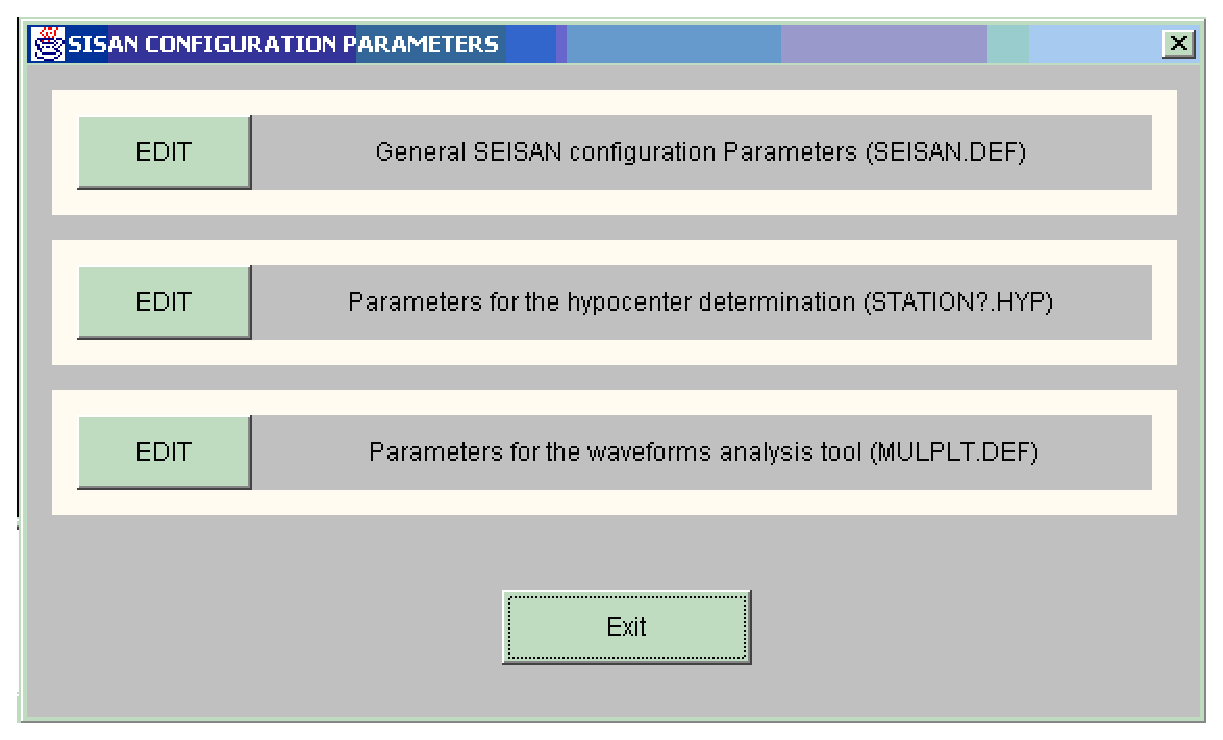
\includegraphics[width=0.9\linewidth]{fig/fig2}}
%\centerline{\includegraphics[width=0.9\linewidth]{fig/fig2.ps}}
\caption{Main Window of the program.}
\label{fig:main-window}
\end{figure}

\textbf{Changing SEISAN.DEF}

The editing process is based on a list made up with the configuration 
parameters. The parameters which are present in the configuration 
file are marked with ``*'' (Figure \ref{fig:main-window}). Parameters 
that are not found in the file, are set to defaults values. These 
default values are taken from the file \texttt{SEISANDEF.INP}. The user 
navigates through the list and can edit the associated values by using 
the edit-boxes labelled as VALUE1 and VALUE2. The entered data is 
validated according to the type and allowed range of values. The check-box 
labelled as ``Use'' permits to select/unselect the selected parameter 
to be saved in the configuration file. The button $<$Add New$> $ allows 
add a new parameter, same type of the one selected in the list, if 
possible. A brief description about the meaning of the selected parameter 
is given at the bottom of the window. 

\begin{figure}
\htmlimage{scale=2.0}
\centerline{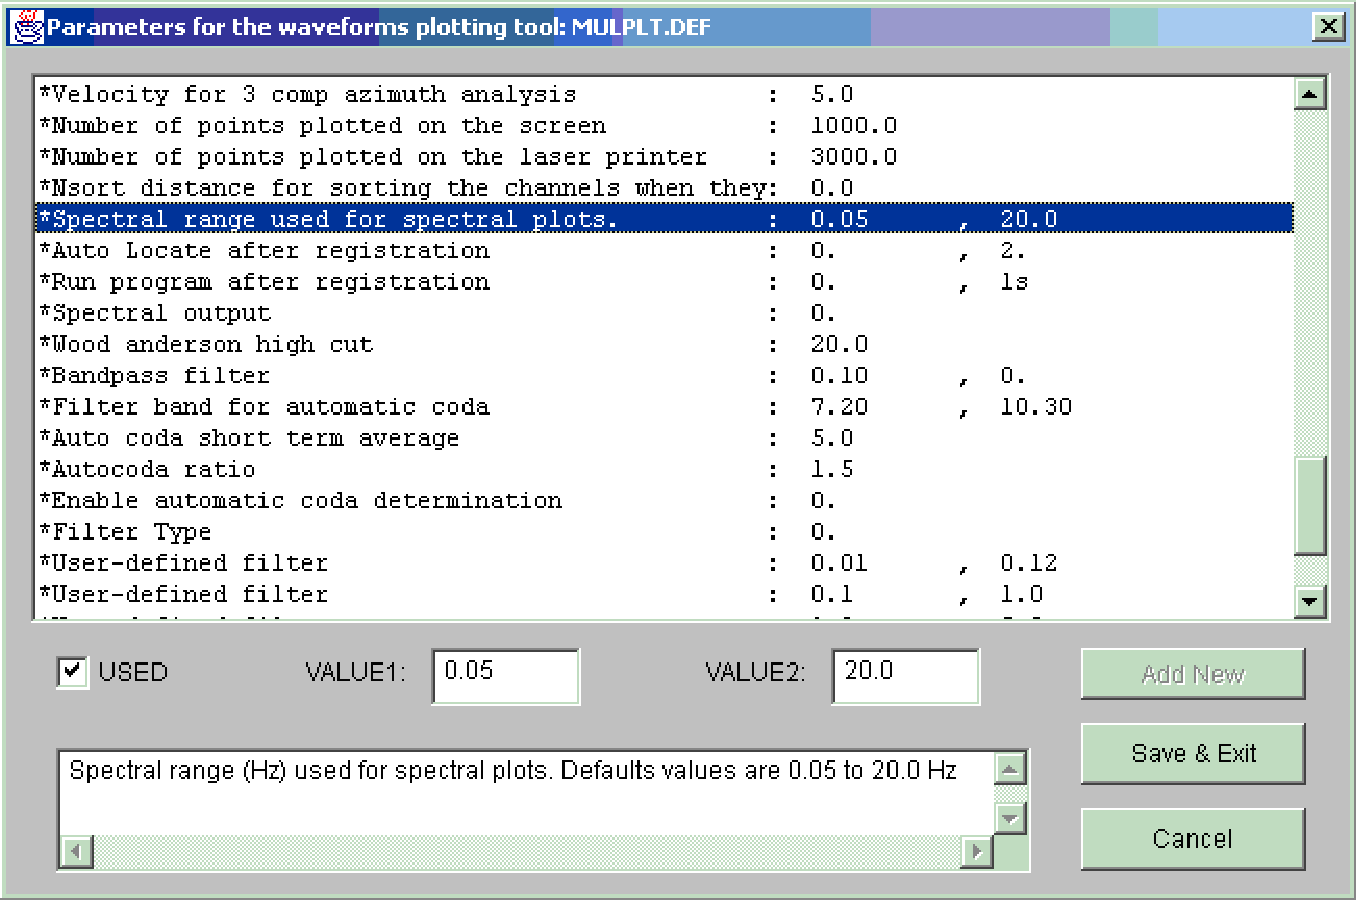
\includegraphics[width=0.9\linewidth]{fig/fig3}}
\caption{Edit Window of the configuration file: \texttt{MULPLT.DEF}}
\label{fig:edit-mulplt.def}
\end{figure}

\textbf{Changing STATION?.HYP}

The editing window (Figure \ref{fig:edit-mulplt.def}) is composed of 
four blocks: (1) A list with the general parameters (RESET TEST) of 
the HYPOCENTER program, (2) The seismic stations list, (3) The velocity 
model and (4) The control line. In addition there is a edit-box for 
the reporting agency and a combo-box labelled as \"Model\" for selecting 
which \texttt{STATION?.HYP} file is being edited. The question mark (?) in the 
file name takes the value selected in the combo-box. By default, 
\texttt{STATION0.HYP} is selected. The combo-box is made up from the set of 
station files (\texttt{STATION?.HYP}) found in the DAT directory or in the 
current local directory. There is two buttons $<$add$>$ and $<$remove$>$ 
in the station list block and velocity model block. Their function 
is for adding or removing items from the list. If you want to add 
a new item and there is one already selected (highlighted), you must 
click the button $<$add$>$ and then change the value with the new one. 
Do not try to enter the data before clicking the button $<$add$>$ 
because that will modify the current value of the selected item. The 
editing process is similar as it was explained in the previous section, 
except that the data for validation and on-line help is taken from 
the file \texttt{STATIONDEF.INP}. 


\begin{figure}
\htmlimage{scale=2.0}
\centerline{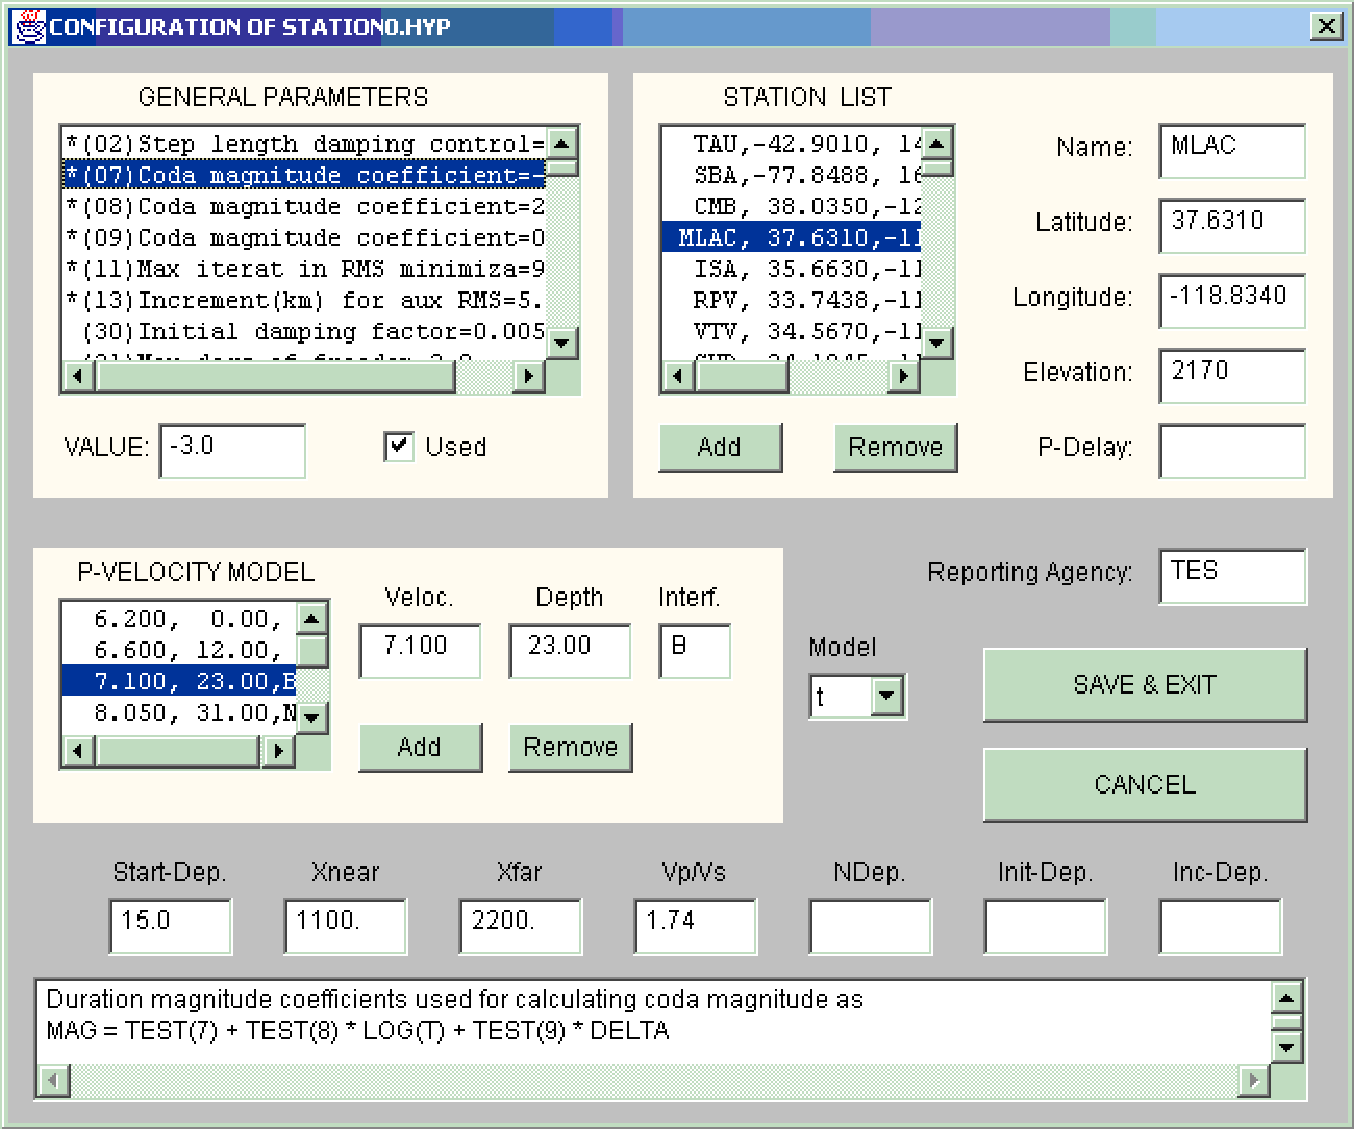
\includegraphics[width=0.9\linewidth]{fig/fig4}}
\caption{Edit Window of the configuration file: \texttt{STATION0.HYP}}
%\label{fig:}
\end{figure}

\textbf{Changing \texttt{MULPLT.DEF}}

The changing is the similar to \texttt{SEISAN.DEF}. The data for validation 
and on-line help is taken from \texttt{MULPLTDEF.INP}. 

\textbf{Input definition file format}

The input files \texttt{SEISANDEF.INP}, \texttt{MULPLTDEF.INP} and 
\texttt{STATIONDEF.INP} are used for data validation purpose and 
user's help support. Normally the user will not edit these files. The first two lines of the files are comments followed by three or more lines for each parameter: (1) The data numerical description, (2) The name and a short description of the parameter shown on the list and 
(3) A longer description (help) about the meaning of the parameter(s). This can be several lines. The data numerical description has the following format: 

$<$Keyword$>$:$<$default$>$,$<$range$>$,$<$value1$>$,$<$value2$>$,...;$<$type$>$,$<$column$>$,$<$width$>$,$<$dec$>$|... 

$<$keyword$>$: Identify the name of the parameter used in the configuration file.\newline
$<$default$>$: Default value used when the parameter is not found in the configuration file.\newline
$<$range$>$: A character for specifying when the parameter is enclosed by a range of values or is allowed to take a set of values. It is set with `R' for range or `U' for a set (see example below). \newline
$<$value1$>$,$<$value2$>$: Represent the lower and upper limit of the range of values which are allow to be 
taken. It is make sense when `R' is used in the $<$range$>$ option. When using `U', then newline
$<$value1$>$,$<$value2$>$,..,$<$valueN$>$ are the set of permitted values. \newline
$<$type$>$: A character for identifying the type of data: `F' float,`I' integer,`S' string of characters. \newline
$<$column$>$: The position (column) of the parameter in the configuration file. \newline
$<$width$>$: The number of characters occupied in the configuration file. \newline
$<$dec$>$: The number of digits after the point for float values. 

When more than one value is taken for a particular parameter, then the character `$|$' is used for 
dividing the two formats. 

Examples: 

SPECTRAL F-BAND:0.05,R,0,20 ; F,40,5,2 | 20.0,R,0,20 ; F,50,5,2 

The keyword \"SPECTRL F-BAND\" has two values. The first one is set by default to 0.05 Hz and can take values between 0 and 20 Hz. It is a float value found in the column 40 of the configuration file and occupies 5 characters with 2 decimal digits. The second value is set by default to 20 Hz and has the same numerical format as the first one, except that it is found in  column 50 of the configuration file. 

MAP\_SERVER:0,U,0,1,2,3,4,5 ; I,40,1 

The keyword \"MAP\_SERVER\" is set by default to 0 and can only take the values 0,1,2,3,4 and 5. It is 
an integer data found in column 40 and occupies a 1 character position. 

WAVEFORM\_BASE:BER ; S,40,5 

The keyword \"WAVEFORM\_BASE\" is set by default to \"BER\". It is a string with a maximum of 5 characters and it is found in the column 40 of the configuration file. 

Below is shown part of the content of \texttt{MULPLTDEF.INP} 

\verbatiminput{include/MULPLTDEF.INP}





